\section*{Methodology}

\begin{figure*}[ht]
\centering
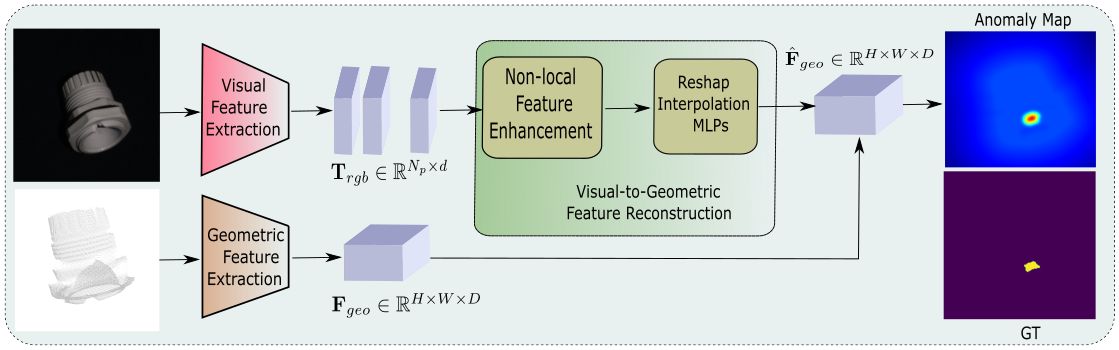
\includegraphics[width=\linewidth]{figs/overview}
\caption{Overview of the proposed unsupervised anomaly detection framework. The method extracts 2D visual features from RGB images and 3D geometric features from point clouds. A Visual-to-Geometric Feature Reconstruction network predicts geometric features from visual inputs, and significant discrepancies indicate anomalies.}
\label{fig:view}
\end{figure*}

Let $\mathbf{I} \in \mathbb{R}^{H \times W \times 3}$ represent an RGB image, where $H$ and $W$ denote the height and width of the image, and the 3 channels correspond to the color information. Let $\mathbf{D} \in \mathbb{R}^{H \times W}$ represent the corresponding depth image, which is pixel-registered with $\mathbf{I}$. This means that each pixel $(u, v)$ in $\mathbf{D}$ corresponds to a pixel in $\mathbf{I}$, providing a depth value $d_{u,v}$ for each valid pixel. From the depth image $\mathbf{D}$, we generate a 3D point cloud $\mathbf{P} = \{(x_i, y_i, z_i)\}_{i=1}^{M}$, where $M$ is the number of valid depth points and each point $(x_i, y_i, z_i)$ represents the 3D coordinates derived from the depth information.

As shown in Figure \ref{fig:view} the objective of the proposed method is to detect anomalies by predicting the 3D geometric features $\hat{\mathbf{F}}_{geo}$ from the 2D visual features $\mathbf{F}_{vis}$ and comparing them with the actual geometric features $\mathbf{F}_{geo}$ extracted from the point cloud. First, the visual features $\mathbf{F}_{vis} \in \mathbb{R}^{H \times W \times d}$ are extracted from the RGB image $\mathbf{I}$ using a Vision Transformer (ViT), capturing the appearance of the object in 2D space. Then, the 3D geometric features $\mathbf{F}_{geo} \in \mathbb{R}^{H \times W \times d}$ are obtained from the depth image $\mathbf{D}$ using a pre-trained 3D model. The core of the method is the geometric feature reconstruction network, which predicts the geometric features $\hat{\mathbf{F}}_{geo}$ from the visual inputs $\mathbf{F}_{vis}$. During training, the network minimizes the difference between the predicted geometric features $\hat{\mathbf{F}}_{geo}$ and the actual geometric features $\mathbf{F}_{geo}$ by minimizing the loss $\mathcal{L}_{geo}$. This process allows the network to learn the normal correlations between 2D visual data and 3D geometric data. During inference, anomalies are detected by comparing the predicted geometric features $\hat{\mathbf{F}}_{geo}$ with the actual geometric features $\mathbf{F}_{geo}$. Significant deviations between these features, measured using the Euclidean distance or another discrepancy measure, indicate abnormal regions in the object.

\subsection*{3D Point Cloud Feature Extraction}

The 3D point cloud $\mathbf{P} = \{(x_i, y_i, z_i)\}_{i=1}^{M}$ is processed using a Masked Autoencoder (MAE) \cite{pang2022masked}. The point cloud is first divided into patches using Farthest Point Sampling (FPS) and K-Nearest Neighbors (KNN). FPS selects $n$ points as patch centers, and KNN selects the $k$ nearest neighbors for each center:

\begin{equation}
    \mathbf{C_T} = \text{FPS}(\mathbf{P}), \quad \mathbf{C_T} \in \mathbb{R}^{n \times 3}.
\end{equation}
\begin{equation}
    \mathbf{P}_{patch} = \text{KNN}(\mathbf{P}, \mathbf{C_T}), \quad \mathbf{P}_{patch} \in \mathbb{R}^{n \times k \times 3}.
\end{equation}

\noindent The masked point patches are processed through PointNet \cite{qi2017pointnet} and the autoencoder to produce geometric features $\mathbf{G}_{geom} \in \mathbb{R}^{M \times D}$. The geometric features $\mathbf{G}_{geom} \in \mathbb{R}^{M \times d}$ are produced for each point in the point cloud. Since the 3D point cloud is derived from the depth image $\mathbf{D}$, we know the pixel coordinates $(u_i, v_i)$ of each 3D point $(x_i, y_i, z_i)$, allowing us to map the geometric features back to their corresponding pixel locations in the 2D image. Using this projection, we place the geometric features into a sparse 2D feature map $\mathbf{G}_{map} \in \mathbb{R}^{H \times W \times d}$, where the pixel $(u_i, v_i)$ contains the feature vector for point $i$.

\begin{equation}
\mathbf{G}_{map}[u_i, v_i, :] = \mathbf{G}_{geom}[i, :].
\end{equation}

\noindent For pixels without corresponding 3D points, we apply interpolation method as in \cite{wang2023multimodal} to propagate geometric features from neighboring pixels:

\begin{equation}
    \mathbf{F}_{geo} = \text{Interpolate}(\mathbf{G}_{map}) \in \mathbb{R}^{H \times W \times D}.
\end{equation}

\subsection*{Visual Feature Extraction}

The RGB image $\mathbf{I}$ is processed using a Vision Transformer (ViT) \cite{dosovitskiy2020image} to extract high-level visual features. The image $\mathbf{I}$ is divided into non-overlapping patches of size $p \times p$, and each patch is flattened into a vector. A linear projection is applied to embed the patches into a $d$-dimensional feature space:

\begin{equation}
    \mathbf{x}_p = \text{Flatten}(\mathbf{I}) \in \mathbb{R}^{(H \times W) / p^2 \times (p \times p \times 3)}.
\end{equation}

\noindent The set of embedded patches is passed through the transformer encoder to obtain RGB feature tokens:

\begin{equation}
    \mathbf{T}_{rgb} = ViT(\mathbf{x}_p) \in \mathbb{R}^{N_p \times d},
\end{equation}

\noindent where $N_p = \frac{H \times W}{p^2}$ is the number of patches and $d$ is the dimension of the feature vectors. 

\subsection*{Visual-to-Geometric Feature Reconstruction}

\begin{figure*}[ht]
\centering
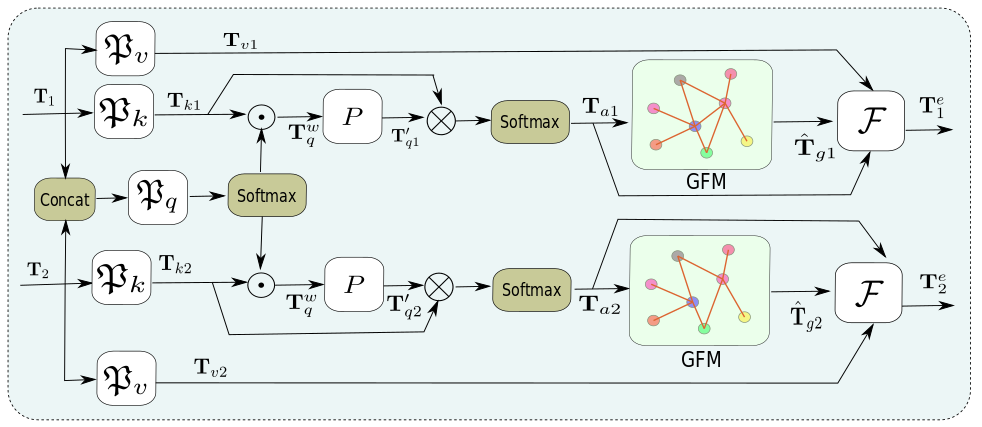
\includegraphics[width=0.8\linewidth]{figs/NL}
\caption{The proposed visual feature enhancement module $\mathcal{M}_{FE}$ used in geometric feature reconstruction. The module incorporates non-local attention and graph convolutional networks to improve the interaction between global and local features.}
\label{fig:NL}
\end{figure*}

The Visual-to-Geometric Feature Reconstruction network serves as the core of the proposed method, learning to reconstruct 3D geometric features from 2D visual inputs. This approach leverages the complementary nature of appearance and geometric information, enabling precise anomaly detection without the need for direct multimodal fusion. 

Transformers are well-suited for capturing global contextual information across visual tokens; however, their ability to model localized interactions remains limited. This limitation is particularly critical in anomaly detection, where fine-grained deviations often indicate defects. To address this, we integrate a visual feature enhancement module $\mathcal{M}_{FE}$ (Figure~\ref{fig:NL}) within the reconstruction network. This module enhances local feature representations while retaining global context by combining non-local attention \cite{wang2018non} with graph convolutional networks (GCNs) \cite{defferrard2016convolutional, te2020edge}. The combination of non-local attention and graph convolutional networks (GCNs) was chosen to effectively address the complementary aspects of global and local feature integration. Non-local attention captures long-range dependencies across the entire image, which is critical for identifying correlations in visual features across spatially distant regions. GCNs, on the other hand, excel at modeling local relationships and refining features based on neighborhood structures.

\paragraph*{Non-Local Attention for Global Context}
Non-local attention \cite{wang2018non} captures relationships between spatially distant visual tokens, providing the network with a global understanding of correlations in visual features. Specifically, given two neighboring tokens $\mathbf{T}_1$ and $\mathbf{T}_2$ extracted from a Vision Transformer, the attention mechanism refines $\mathbf{T}_1$ as follows:

\begin{equation}
\mathbf{T}_v = \mathfrak{P}_v(\mathbf{T}_1), \quad \mathbf{T}_k = \mathfrak{P}_k(\mathbf{T}_1),
\end{equation}

\noindent where $\mathfrak{P}_v$ and $\mathfrak{P}_k$ are linear projection layers reducing the dimensionality of $\mathbf{T}_1$ to $\frac{d}{2}$. $\mathbf{T}_1$ and $\mathbf{T}_2$ are concatenated to form $\mathbf{T}_q$, and the attention weights are computed as:

\begin{equation}
\mathbf{T}_q^w = \text{softmax}(\mathfrak{P}_q(\mathbf{T}_q)), \quad \mathbf{T}_q' = P\left(\mathbf{T}_k \odot \mathbf{T}_q^w\right),
\end{equation}

\noindent where $\mathfrak{P}_q$ projects $\mathbf{T}_q$ to a lower dimension, and $P(\cdot)$ is adaptive average pooling. The attention map $\mathbf{T}_a$ is derived from the interaction:

\begin{equation}
\mathbf{T}_a = \text{softmax}(\mathbf{T}_q' \otimes \mathbf{T}_k^\top).
\end{equation}

\paragraph*{Graph Convolutional Networks for Local Interactions}
Local interactions between visual features are refined using a graph convolutional network (GCN) \cite{te2020edge}. Tokens are projected into a graph representation where vertices represent similar features, and edges encode relationships. The refined token $\hat{\mathbf{T}}_g$ is computed as:

\begin{equation}
\hat{\mathbf{T}}_g = \text{ReLU}\left((I - A)\mathbf{T}_g w_g\right),
\end{equation}

\noindent where $\mathbf{T}_g = \mathbf{T}_v \otimes \mathbf{T}_a^\top$, $A$ is the adjacency matrix, and $w_g$ is the GCN weight matrix. A skip connection integrates global and local refinements:

\begin{equation}
\mathbf{T}_1^e = \hat{\mathbf{T}}_g + \mathbf{T}_1.
\end{equation}

\noindent The same process is applied to other tokens. The adjacency matrix $A$ is dynamically constructed based on the similarity of visual tokens in the feature space. Specifically, token similarity is measured using a distance metric, and a thresholding mechanism is applied to determine graph connectivity. This approach ensures that $A$ adapts to the characteristics of each input, capturing relevant local relationships. The GCN's ability to model higher-order interactions and propagate contextual information across connected nodes provides a distinct advantage over simpler feature aggregation methods, particularly in capturing subtle anomalies that span localized regions.

\paragraph*{Reconstruction of Geometric Features}
The enhanced visual features $\mathbf{T}^e$ are reshaped and upsampled to match the spatial dimensions of the input image:

\begin{equation}
\mathbf{F}_{patches} = \text{Reshape}(\mathbf{T}^e) \in \mathbb{R}^{\frac{H}{p} \times \frac{W}{p} \times d},
\end{equation}

\begin{equation}
\mathbf{F}_{vis} = \text{BilinearUpsample}(\mathbf{F}_{patches}) \in \mathbb{R}^{H \times W \times d}.
\end{equation}

\noindent Bilinear upsampling was selected for its simplicity and computational efficiency. While more complex methods, such as learnable upsampling, could potentially improve alignment precision, experiments showed that bilinear upsampling produced negligible artifacts and did not significantly affect the accuracy of the reconstructed geometric features. Finally, $\mathbf{F}_{vis}$ is passed through a lightweight MLP to predict geometric features $\hat{\mathbf{F}}_{geo}$:

\begin{equation}
\hat{\mathbf{F}}_{geo} = \text{MLP}(\mathbf{F}_{vis}).
\end{equation}

\paragraph*{Loss Function}
The network minimizes the L2 reconstruction loss to align the predicted geometric features $\hat{\mathbf{F}}_{geo}$ with the ground-truth features $\mathbf{F}_{geo}$:

\begin{equation}
\mathcal{L}_{geo} = \frac{1}{HWD} \sum_{i=1}^{H} \sum_{j=1}^{W} \sum_{k=1}^{D} \left( \mathbf{F}_{geo}(i, j, k) - \hat{\mathbf{F}}_{geo}(i, j, k) \right)^2.
\end{equation}

\noindent By leveraging non-local attention and GCNs, $\mathcal{M}_{FE}$ ensures effective integration of global and local information. This design allows the network to capture subtle deviations in both texture and geometry, resulting in accurate anomaly detection for complex industrial settings.

\subsection*{Anomaly Localization}

During inference, we use the trained prediction network to predict geometric features from the visual features of test samples. For each sample, we extract the 2D visual features $\mathbf{F}_{vis}$ from the RGB image using the pre-trained 2D model and the 3D geometric features $\mathbf{F}_{geo}$ from the point cloud using the pre-trained 3D model. The visual features $\mathbf{F}_{vis}$ are then passed through the geometric feature prediction network to predict the corresponding geometric features $\hat{\mathbf{F}}_{geo}$. We compute an anomaly map by measuring the difference between the predicted geometric features $\hat{\mathbf{F}}_{geo}$ and the actual geometric features $\mathbf{F}_{geo}$ at each spatial location using the L2 norm:

\begin{equation}
\mathbf{A}_{\text{anomaly}}(i, j) = \|\mathbf{F}_{geo}(i, j) - \hat{\mathbf{F}}_{geo}(i, j)\|_2.
\end{equation}

\noindent This anomaly map $\mathbf{A}_{\text{anomaly}} \in \mathbb{R}^{H \times W}$ indicates the likelihood of anomalies at each spatial location. Regions with higher values represent areas where the predicted geometric features deviate significantly from the actual geometric features, suggesting the presence of anomalies. The predicted anomaly map is finally smoothed using a Gaussian kernel with $\sigma$=4, following \cite{roth2022towards}. To obtain a global anomaly score for each sample, we calculate the maximum value in the smoothed anomaly map:

\begin{equation}
S_{\text{global}} = \max_{i,j} \mathbf{A}_{\text{anomaly}}(i, j).
\end{equation}

\noindent If the global anomaly score $S_{global}$ exceeds a predefined threshold, the sample is classified as anomalous. The threshold can be determined as in \cite{bergmann2022mvtec, wang2023multimodal}. Additionally, the anomaly map provides spatial localization of anomalies by highlighting regions where the largest deviations occur, enabling a detailed inspection of the anomalous areas. 
